\chapter{$\chi^2$ - Badanie jakości dopasowania śladów}
Krytycznym punktem każdego eksperymentu fizycznego jest, poza dokonanie niezbędnych pomiarów przeanalizowanie ich. Główne metody analizy danych doświadczalnych bazują na statystyce. W większości przypadków do zebranych danych eksperymentator stara się dopasować pewien model. Dopasowywany model powinien być tak dobrany, aby możliwe było wyznaczenie pewnych, poszukiwanych parametrów. 

Dlatego kluczowym elementem podczas przeprawiania analizy danych powinna być weryfikacja otrzymanych wyników. Niska jakość dopasania modelu do danych przekłada się na fakt, iż otrzymane wyniki są mało wiarygodne. Badanie jakości daje możliwość weryfikacji poprawności wyboru danego modelu. Głównym narzędziem służącym do tego jest test $\chi^2$.


\section{Definicja $\chi^2$}

Niech próbka zawiera $\nu$  niezależnych zmiennych $x_i$  pochodzących z rozkładów normalnych o średnich $\mu_i$ oraz wariancjach $\sigma_i$, to wielkość nazywana $\chi^2$ \footnote{Warto zwrócić uwagę, że używana nazwa $\chi^2$ może być myląca, gdyż jest to pojedyncza statystyczna zmienna a nie kwadrat jakiejś wielkości $\chi$. Notacja ta powinna być rozumiana w sensie, że wielkość ta składa się z sumy kwadratów.} jest definiowana jako

\begin{eqnarray}
\chi^2 &=& \frac{(x_1-\mu_1)^2}{\sigma_1^2}+\frac{(x_2-\mu_2)^2}{\sigma_2^2}+\ldots + \frac{(x_\nu-\mu_\nu)^2}{\sigma_\nu^2} \nonumber \\
&=& \sum_{i=0}^{\nu}\frac{(x_i-\mu_i)^2}{\sigma_i^2}
\label{chiRownanie}
\end{eqnarray}

W idealnym przypadku, po uwzględnieniu przypadkowych fluktuacji każdy z czynników sumy \ref{chiRownanie} powinien być rzędu jedności. Zatem przy założeniu dobrania odpowiednich wartości  $\mu_i$ oraz $\sigma_i$ powinno się spodziewać, że obliczona wartość $\chi^2$ powinna się zbliżać do $\nu$. Jeżeli tak jest, to uzasadnione jest wyciągnięcie wniosku, że dane opisane są dobrze przez wartości $\mu_i$ czyli innymi słowami hipotetyczną funkcję. 
Z drugiej strony, jeżeli wartość sumy $\chi^2$ znacznie odbiega od $\nu$ prawdopodobnie wybrany model nie opisuje zbyt dokładnie zmierzonych danych. 

Powyżej przedstawiono ogólną idee stojącą za testem $\chi^2$. W następnych częściach tego rozdziału omówione jak wygląda procedura przeprowadzania takiego testu.

\section{Rozkład $\chi^2$}

Wielkość  $\chi^2$ zdefiniowana równaniem \ref{chiRownanie} posiada funkcję gęstości prawdopodobieństwa daną równaniem: 

\begin{equation}
f(\chi^2)=\frac{1}{2^{0.5 \nu} \Gamma(\frac{\nu}{2})}e^{\frac{\nu^2}{2}} \left( \chi^2 \right)^{\frac{\nu^2}{2}-1}
\label{chi2Dis}
\end{equation}

Funkcja przedstawiona powyżej (równanie \ref{chiRownanie}) zwana jest rozkładem  $\chi^2$  o $\nu$ stopniach swobody, przy czym $\nu \in \mathbb{N}_{+}$. Na rysunku \ref{fig:chi2} zamieszczony został ten rozkład dla kilku, wybranych stopni swobody. 

\begin{figure}[h]
  \centering
  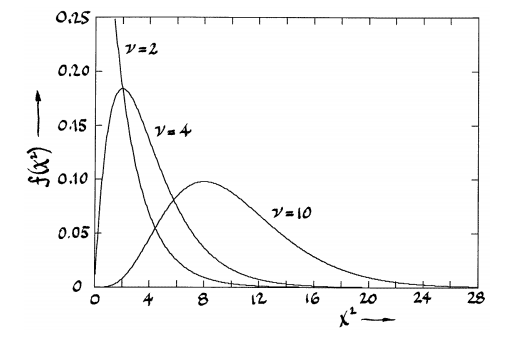
\includegraphics[scale=0.7]{rozdzial5/chi2.png}
  % AccComple.gif: 480x434 pixel, 72dpi, 16.93x15.31 cm, bb=0 0 480 434
  \caption{Funkcja rozkładu prawdopodobieństwa $\chi^2$  dla $\nu=2,4,10$.}
  \label{fig:chi2}
\end{figure}

Warto zwrócić uwagę na wartości parametrów tego rozkładu. Średnia wartość rozkładu $\chi^{2}_{\nu}$ wynosi $\nu$, natomiast wariancja jest równa $2\nu$. Łatwo jest również zauważyć, że rozkład ma dużą dodatnią skośność, która to zmienia się wraz z wartością parametru $\nu$, stając coraz mniejszą dla coraz to większych wartości ilości stopni swobody. Fakt ten wynika z centralnego twierdzenia granicznego.
\section{Sposób wykorzystania testu $\chi^2$ do badania jakości dopasowania} 

Niech próbka pomiarowa składa się z N pomiarów eksperymentalnych pewnych wielkości $x_i$. Eksperymentator chce sprawdzić, czy dane te są dobrze opisane przez zbiór hipotetycznych wartości $\mu_i$. W tym celu formułuje sumę zgodnie z równaniem \ref{chiRownanie}. Warto zwrócić uwagę, iż bardzo istotnym faktem, po za samym pomiarem jest wyznaczenie niezależnie dla każdego pomiaru niepewności $\sigma_i$. 

Powtarzając ten eksperyment wiele razy oraz za każdym razem konstruując sumę $\chi^2$ doświadczalnik powinien spodziewać się, ~o ile model którego używa jest prawidłowy, że rozkład sum będzie się zachowywał zgodnie z równaniem \ref{chi2Dis}. W tym momencie warto być ostrożnym, ponieważ ilość stopni swobody nie musi być, i zazwyczaj nie jest równa ilości punktów pomiarowych. Ilość stopni swobody jest równa ilości punktów pomiarowych pomniejszona o ilość estymowanych parametrów modelu. 

Metody statystyczne nie są w stanie odpowiedzieć na pytanie czy dany model jest poprawny czy nie. Może, natomiast podać odpowiedz na pytanie w jakim przedziale istotności $\alpha$ wybrany przez eksperymentatora model dobrze opisuje zbiór danych pomiarowych. Z matematycznego punktu widzenia przedział istotności opisany jest równaniem:
\begin{equation}
\alpha=\int^{\infty}_{\chi^2_{\nu,\alpha}}f(\chi^2)d\chi^2
\end{equation}

Z praktycznego punktu widzenia w celu weryfikacji hipotezy o poprawności danego modelu trzeba najpierw obliczyć wartość znormalizowanej sumy $\chi^2 \slash \nu $ a następnie porównać ją z wartością $\chi^2_{\nu,\alpha} \slash \nu $. Jeżeli otrzymana wartość jest większa może to oznaczać:
\begin{itemize}
\item wybrany model niedostatecznie opisuje dane doświadczalne, 
\item model jest prawidłowy zaszło zdarzenie statystycznie mało prawdopodobne. 
\end{itemize}

Warto zwrócić uwagę na pewne założenie dotyczące rozkładu zmiennych losowych. Cała idea sumy $\chi^2$ bazuje na założeniu o rozkładzie Gaussa. W związku z tym pewne punkty pomiarowe znacząco odbiegające od rozkładu normalnego mogą znacząco podnieść wartość sumy. 

Drugim, skrajnym przypadkiem są ''dane za dobre''. Taka sytuacja może być spowodowana przykładowo złą estymacją wartości $\sigma_i$. Warto zapamiętać, że zbyt mała wartość nie jest związana ze niską jakością modelu opisującego dane, taki model może tylko podnosić wartość sumy $\chi^2$. 
